\documentclass{article}
\usepackage{color}
\usepackage{graphicx}
\usepackage{setspace}
\usepackage{hyperref}
\usepackage{geometry}
\usepackage{amsmath}
\usepackage{enumitem,amssymb}
\usepackage{pifont}
\definecolor{darkgreen}{rgb}{0.0, 0.5, 0.0}
\geometry{left = 1.25in, right=1.25in} % New Stuff Learned!
\newcommand{\cmark}{\ding{51}}
\newcommand{\xmark}{\ding{55}}
\newcommand{\done}{\rlap{$\square$}{\raisebox{2pt}{\large\hspace{1pt}\cmark}}
\hspace{-2.5pt}}
\newcommand{\wontfix}{\rlap{$\square$}{\large\hspace{1pt}\xmark}}
\newlist{todolist}{itemize}{2}
\setlist[todolist]{label=$\square$}
\doublespacing
\begin{document}
\begin{titlepage}

\title{\textbf{CHE374 Week 1}}
\author{\textit{Sanzhe Feng}}
\date{\textit{\today}}
\maketitle
\end{titlepage}
\setlength{\parindent}{0pt}

\section*{Motivation of Unsupervised Learning}
Usually, it is hard and expensive to collect labeled data required for supervised learning.

- Generative modeling

- Self-supervised learning

- Compression

In this course, we will be looking at three applications of unsupervised learning:

- Clustering: recommendation/search results, marktet segmentation, social network analysis

- Dimensionality reduction: get rid of redundancy

- Data visualization

\section*{Clustering with the k-means algorithm}

k-mean algorithm is used to find the clusters of data.

First, randomly select two cluster centroids. Compute the distance between the each data to the centroids, then we assign each data point to the centroid that is closest to it.

Then we update the location of the centroids by computing the mean of all the points that have been assigned to each cluster. 

Reset all data points to be unassigned. Repeat the distance calculation and the relocation of centroids. 


\subsection*{k-mean algorithm}
- input: k number of clusters; training set $\{x^{1}...x^{n}\}$

- random initialization: k cluser centroids $\mu_1...\mu_k$

- Repeat: 
    for i in 1 to m

    \hspace{1.1cm}$c^{(i)}$ = index of cluster centroid closest to $x^i$

    for k in 1 to k

    \hspace{1.1cm}$\mu_k$ = mean of points assigned to cluseter k


\section*{Distortion in the k-means algorithm}

\subsection*{Optimization objective }
Cost function: $J(c^1, ... , c^m, \mu_1, ..., \mu_u) = \frac{1}{m}\sum ||x^i -\mu_c||^2$

2 steps of k-mean algorithms:

1. Cluster assignment step: minimizing cost function wrt to c while fixing $\mu$

2. Move centroids step: minimizing cost function wrt $\mu$ while fixing c

\subsection*{Initialization}
How to pick the value of K:

                            
Strategy is to pick random points as K in the input domain or K training sets as the K initial cluster centroids. 

\subsection*{Local Optima}
Problem that caused by initialization. 

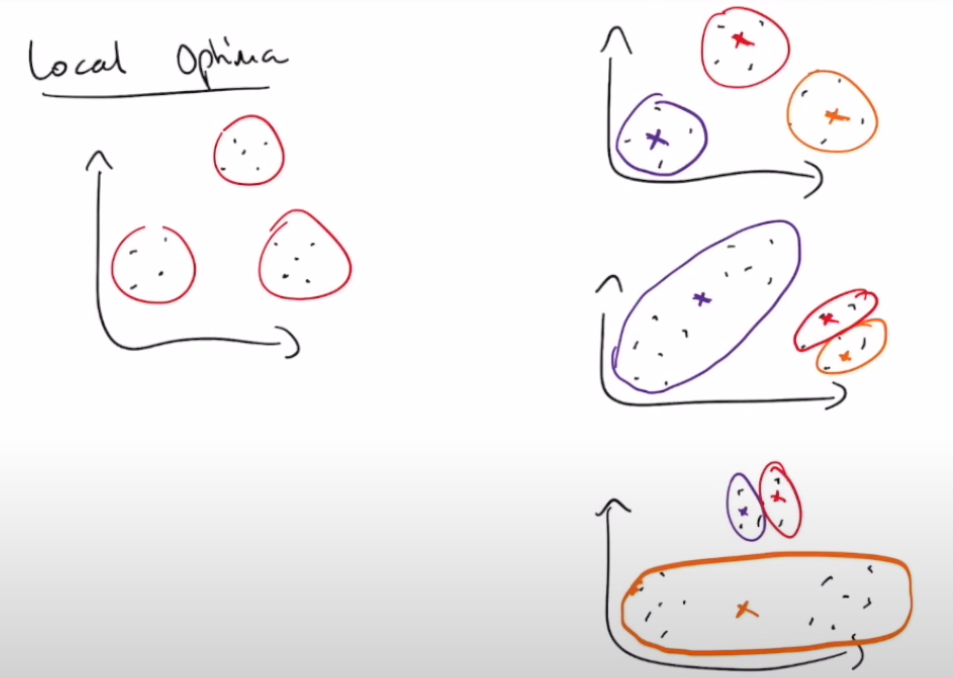
\includegraphics[width=0.7\linewidth]{W2V3.png}

- For some number of trials, randomly initialize k centroids, $\mu_1 ... \mu_k$, then run k means to obtain $c_1,...c_n, mu_1...mu_k$
to compute distortion/cost J. Pick random initialization that yileds min J
then we pick the results yield by that J.

When we increase the value of k, we measure the distortion. The inflection point may be a good choice for the value k picked.

\section*{Principal Component Analysis (PCA)}
We use PCA to make data in 2D into 1D (Compression): Find a vector, minimize the projection error (the distance between the point and the vector). In general, if we want to reduce from nD to kD, we need k vectors.\\


Linear regression and PCA: In linear regression, rather than projection, it is the vertical line(to x-axis) between data and the line. In PCA, it is the vertical line to the vector. \\

PCA Algorithm:

Preprocessing: input training sets x from 1 to m;
Mean normalization: $\mu = \frac{1}{\mu}\sum_{i=1}^m x_j^{(i)}$, then take $x_j$ to be $x_j - \mu_j$
Feature Scaling: scale features to have comparable ranges of values. 

Scale: S_j; Replace $x_j$ with $\frac{x_j^i - \mu_j}{S_j}$

i: index of the data in the training set; 

J: index of the feature, (n dimensions, n features)

Algorithm: (nD->kD)

1. Compute covariance matrix:
\[\Sigma = \frac{1}{\mu} sum_{i=1}^M (x^i)(x^i)^T
This gives a nxn matrix.

2.Compute eigenvectors sigma
$U,S,V =$ singular value decomposition ($\Sigma $)
U: a matrixs contains columns that we are looking for. First k columns are what we need previously.

Project x to z, z is a matrix with columns u
$z^T x$ successfully project x to z (z transpose is k * n matrix, x is n * 1). 

Reversely, $x = U_{[1-k]}^T x. The data will be still on the line (error comes from compression). But we successfuly convert 1D to 2D.

How do we choose K: 

average squared projection error:
$\frac{1}{\mu} \sum_{i=1}^M ||x^i - x_{aprrox}^i||^2$

Total variance in the data: $\frac{1}{\mu}\sum_{i=1}^M ||x||^2

Choose k s.t. the ratio between these two $\leq 0.01$ Since 99.9% of data is retained.

Application/Tips on PCA
-Data compression
-Visualization
-Speed-up learning


\end{document}
